\documentclass[10pt,landscape,a4paper]{article}
\usepackage{multicol}
\usepackage[landscape]{geometry}
\usepackage{hyperref}
\usepackage[utf8]{inputenc}
\usepackage{minted}
\usepackage{graphicx}
\usepackage{graphicx}


\geometry{top=0.5cm,left=0.5cm,right=0.5cm,bottom=0.5cm}

% Turn off header and footer
\pagestyle{empty}
 
% Redefine section commands to use less space
\makeatletter
\renewcommand{\section}{\@startsection{section}{1}{0mm}%
                                {-1ex plus -.5ex minus -.2ex}%
                                {0.5ex plus .2ex}%x
                                {\normalfont\large\bfseries}}
\renewcommand{\subsection}{\@startsection{subsection}{2}{0mm}%
                                {-1explus -.5ex minus -.2ex}%
                                {0.5ex plus .2ex}%
                                {\normalfont\small\bfseries}}
\renewcommand{\subsubsection}{\@startsection{subsubsection}{3}{0mm}%
                                {-1ex plus -.5ex minus -.2ex}%
                                {1ex plus .2ex}%
                                {\normalfont\footnotesize\bfseries}}
\makeatother

% Don't print section numbers
\setcounter{secnumdepth}{0}

\setlength{\parindent}{0pt}
\setlength{\parskip}{0pt plus 0.5ex}

% -----------------------------------------------------------------------

\newcommand{\tfile}[2]{\section{#2}\inputminted{#1}{../../wed2/WED2-Testat/#2}}
\DeclareUnicodeCharacter{25CF}{$\bullet$}
%\setminted{fontsize=\footnotesize}

\begin{document}

\tiny
\begin{multicols*}{3}


% multicol parameters
% These lengths are set only within the two main columns
%\setlength{\columnseprule}{0.25pt}
\setlength{\premulticols}{1pt}
\setlength{\postmulticols}{1pt}
\setlength{\multicolsep}{1pt}
\setlength{\columnsep}{2pt}


\tfile{js}{controller/createedit.js}
\tfile{js}{controller/list.js}
\tfile{css}{public/stylesheets/style.css}
\tfile{js}{routes/index.js}
\tfile{html+handlebars}{views/create.hbs}
\tfile{html+handlebars}{views/error.hbs}
\tfile{html+handlebars}{views/index.hbs}
\tfile{html+handlebars}{views/layout.hbs}
\tfile{js}{app.js}
\tfile{js}{database.js}

\begin{multicols}{2}
\section{Box sizing}
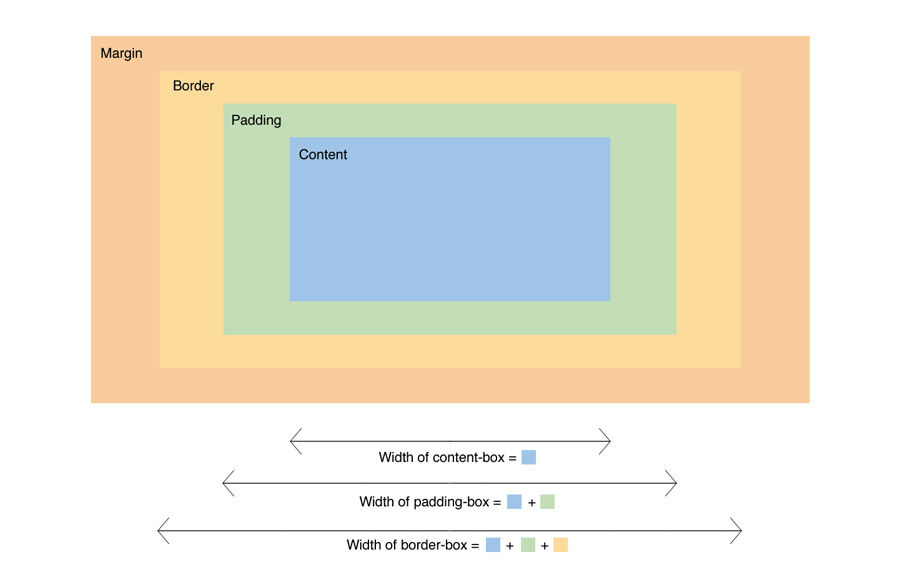
\includegraphics[width=\linewidth]{box-sizing.jpg}
\columnbreak
\section{JS default args}
\begin{minted}{js}
function f1(a = '', b = '*');
// named args
function f2({a = '', b = '*' } = {});
function f3({ a, b } = { a: 1, b: 2 });
// f3({a:5}) -> b undefined
function f4({ a = 1, b = 2} = {});
// f4({a:5}) -> b 2
\end{minted}
\end{multicols}

\section{CSS Grid}

\begin{minted}{css}
#container {
  display: grid;
  grid-template-columns: 25% 100px auto;
  grid-template-rows: 1fr 2fr;
  grid-gap: <grid-row-gap> <grid-column-gap>;
  justify-items: start | end | center | stretch;  /* row axis: lr */
  align-items: start | end | center | stretch;  /* column axis: tb */
  justify-content: start | end | center | stretch | space-around | space-between | space-evenly;	
  align-content: start | end | center | stretch | space-around | space-between | space-evenly;	
}

#item {
  grid-column/row-start/end: <number> | <name> | span <number> | span <name> | auto;
  grid-column: <start-line> / <end-line> | <start-line> / span <value>;
  grid-area: <name> | <row-start> / <column-start> / <row-end> / <column-end>;
  justify-self: start | end | center | stretch;
  align-self: start | end | center | stretch;
}
\end{minted}

\begin{multicols}{2}
\section{Garret}
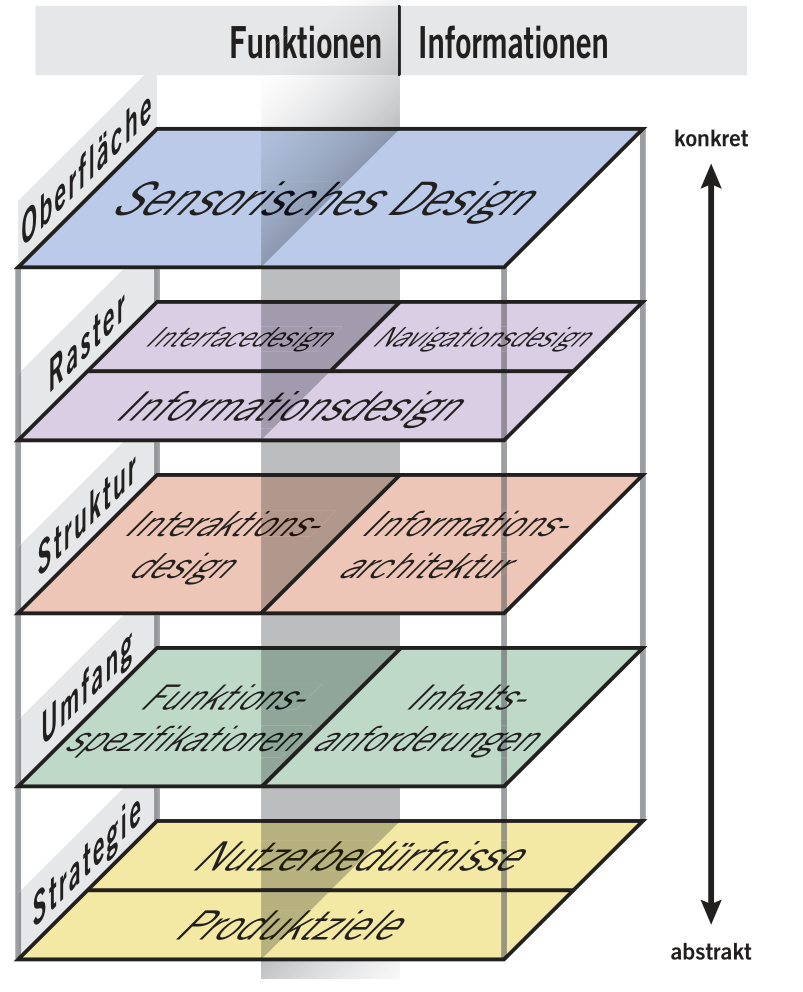
\includegraphics[width=0.8\linewidth]{garret.png}

\section{Visibility/Affordance}
\textbf{Visibility: It Should Be Obvious What a Control Is Used For.} \\
If I press this button, what will happen? If I want to unlock the door, which
control should I use? A system with good visibility allows the user to easily
translate goals into actions. \\
\textbf{Affordance: It Should Be Obvious How a Control Is Used.} \\
The system should provide “strong clues to the operation of things”. A button
affords pushing, a lever affords pulling, etc. The user should know how to
operate a control just by looking at it. \\
\textbf{Feedback: It Should Be Obvious When a Control Has Been Used.} \\
Once the user has pressed a button, the system should react in a manner that clearly communicates what has just been accomplished. If nothing has happened, this fact should also be obvious.
\end{multicols}{2}

\end{multicols*}
\end{document}